%% ----------------------------------------------------------------
%% Thesis.tex -- MAIN FILE (the one that you compile with LaTeX)
%% ---------------------------------------------------------------- 

% Set up the document
\documentclass[a4paper, 11pt, oneside]{Tesi}  % Use the "Thesis" style, based on the ECS Thesis style by Steve Gunn
\graphicspath{{Figure/}}  % Location of the graphics files (set up for graphics to be in PDF format)



% Include any extra LaTeX packages required
\usepackage[utf8]{inputenc}
\usepackage[brazilian]{babel}
\usepackage[T1]{fontenc}
\usepackage{ae,aecompl}
\usepackage[square, numbers, comma, sort&compress]{natbib}  % Use the "Natbib" style for the references in the Bibliography
\usepackage{verbatim}  % Needed for the "comment" environment to make LaTeX comments
\usepackage{vector}  % Allows "\bvec{}" and "\buvec{}" for "blackboard" style bold vectors in maths
%\usepackage{listings}
\usepackage{listingsutf8}
\lstset{frame=tb,
  language=Python,
  aboveskip=3mm,
  belowskip=3mm,
  showstringspaces=false,
  columns=flexible,
  basicstyle={\small\ttfamily},
  numbers=none,
  numberstyle=\tiny\color{gray},
  keywordstyle=\color{dkblue},
  commentstyle=\color{dkgreen},
  stringstyle=\color{mauve},
  breaklines=true,
  breakatwhitespace=true
  tabsize=2
  morekeywords={models, lambda, forms, =}
  inputencoding=utf8,
  extendedchars=\true
}

\lstnewenvironment{code}[1][]%
  {\minipage{\linewidth} 
   \lstset{basicstyle=\ttfamily\footnotesize,frame=tb,#1}}
  {\endminipage}


%%%% Color definitions
\usepackage{color}
\definecolor{dkgreen}{rgb}{0,0.6,0}
\definecolor{dkblue}{rgb}{0,0,0.5}
\definecolor{gray}{rgb}{0.5,0.5,0.5}
\definecolor{mauve}{rgb}{0.6,0,0.82}
\definecolor{coolblack}{rgb}{0.0, 0.18, 0.39}
\hypersetup{urlcolor=coolblack, colorlinks=true}  % Colours hyperlinks in blue, but this can be distracting if there are many links.
%\hypersetup{urlcolor=black, colorlinks=false}  

%% To show a border around all figures
%\usepackage{float}
%\floatstyle{boxed} 
%\restylefloat{figure}

%% ----------------------------------------------------------------
\begin{document}
\frontmatter	  % Begin Roman style (i, ii, iii, iv...) page numbering

% Set up the Title Page
\title  {Redes federadas eventualmente conectadas}

\authors  {\texorpdfstring
            {\href{mailto:vince@mocambos.net}{Vincenzo Tozzi}}
            {Vincenzo Tozzi}
            }
\addresses  {\groupname\\\deptname\\\univname}  % Do not change this here, instead these must be set in the "Thesis.cls" file, please look through it instead
\date       {\today}
\subject    {Tesi di Laurea in Informatica}
\keywords   {Federated Network, Tecnological Autonomy, Free Software, Rede Mocambos, Casa de Cultura Taina, Quilombo}

\maketitle
%% ----------------------------------------------------------------

\setstretch{1.3}  % It is better to have smaller font and larger line spacing than the other way round

% Define the page headers using the FancyHdr package and set up for one-sided printing
\fancyhead{}  % Clears all page headers and footers
\rhead{\thepage}  % Sets the right side header to show the page number
\lhead{}  % Clears the left side page header

\pagestyle{fancy}  % Finally, use the "fancy" page style to implement the FancyHdr headers

% %% ----------------------------------------------------------------
% % Declaration Page required for the Thesis, your institution may give you a different text to place here
% \Declaration{

% \addtocontents{toc}{\vspace{1em}}  % Add a gap in the Contents, for aesthetics

% Io, Vincenzo Tozzi, dichiaro che la presente tesi, "Reti federate eventualmente connesse" e il lavoro presentato in essa sono di mia paternità. Dichiaro che:

% \begin{itemize} 
% \item[\tiny{$\blacksquare$}] Questo lavoro è stato totalmente o per la maggior parte svolto come laureando per la Laurea in Informatica di questa Università.
 
% \item[\tiny{$\blacksquare$}] Ho esplicitamente dichiarato nel testo se qualche parte di questa tesi è stata precedentemente pubblicata in altri lavori da questa o altre Università o istituzioni.
 
% \item[\tiny{$\blacksquare$}] Ho attribuito la paternità ai lavori pubblicati da altri e da me consultati.
 
% \item[\tiny{$\blacksquare$}] Ho sempre citato la fonte di opere altrui. Ad eccezione di tali citazioni, questa tesi è di mia paternità.
 
% \item[\tiny{$\blacksquare$}] Ho ringranziato tutte le principali fonti di supporto.
 
% \item[\tiny{$\blacksquare$}] Ho esplicitamente dichiarato del testo, in parti sviluppate assieme ad altri, qual'è il loro e il mio contributo.
% \\
% \end{itemize}
 
 
% Firmato:\\
% \rule[1em]{25em}{0.5pt}  % This prints a line for the signature
 
% Data:\\
% \rule[1em]{25em}{0.5pt}  % This prints a line to write the date
% }
% \clearpage  % Declaration ended, now start a new page

%% ----------------------------------------------------------------
% The "Funny Quote Page"
\pagestyle{empty}  % No headers or footers for the following pages

\null\vfill
% Now comes the "Funny Quote", written in italics
\textit{``Vamos fazer um mundo mais do nosso jeito\ldots''}

\begin{flushright}
Zumbi dos Palmares
\end{flushright}

\vfill\vfill\vfill\vfill\vfill\vfill\null
\clearpage  % Funny Quote page ended, start a new page
%% ----------------------------------------------------------------

% The Abstract Page
\addtotoc{Abstract}  % Add the "Abstract" page entry to the Contents
\abstract{

\addtocontents{toc}{\vspace{1em}}  % Add a gap in the Contents, for aesthetics

This work researches on technologies for a federated network of
afrodescendants communities looking at autonomy and freedom. The work
propose an architecture and prototype for an eventually connected
federated network where the main limit and technical bond is the
connection availability and bandwidth. The prototype is a media
sharing system for local web portals, based on Django and Git-Annex,
authenticated on LDAP servers.

}

\clearpage  % Abstract ended, start a new page
%% ----------------------------------------------------------------

\setstretch{1.3}  % Reset the line-spacing to 1.3 for body text (if it has changed)

% The Acknowledgements page, for thanking everyone
\acknowledgements{
\addtocontents{toc}{\vspace{1em}}  % Add a gap in the Contents, for aesthetics

Um agradecimento especial para as minha famílias\ldots

}
\clearpage  % End of the Acknowledgements
%% ----------------------------------------------------------------

\pagestyle{fancy}  %The page style headers have been "empty" all this time, now use the "fancy" headers as defined before to bring them back


%% ----------------------------------------------------------------
\lhead{\emph{Contents}}  % Set the left side page header to "Contents"
\tableofcontents  % Write out the Table of Contents

%% ----------------------------------------------------------------
\lhead{\emph{List of Figures}}  % Set the left side page header to "List if Figures"
\listoffigures  % Write out the List of Figures

%% ----------------------------------------------------------------
%\lhead{\emph{List of Tables}}  % Set the left side page header to "List of Tables"
%\listoftables  % Write out the List of Tables

%% ----------------------------------------------------------------
\setstretch{1.5}  % Set the line spacing to 1.5, this makes the following tables easier to read
\clearpage  % Start a new page
\lhead{\emph{Abreviações}}  % Set the left side page header to "Abbreviations"
\listofsymbols{ll}  % Include a list of Abbreviations (a table of two columns)
{
% \textbf{Acronym} & \textbf{W}hat (it) \textbf{S}tands \textbf{F}or \\
  \textbf{GESAC} & \textbf{G}overno \textbf{E}letrônico
  \textbf{S}erviço
  de \textbf{A}tendimento ao \textbf{C}idadão\\
  \textbf{RM} & \textbf{R}ede \textbf{M}ocambos\\
  \textbf{SP} & \textbf{S}ervice \textbf{P}rovider\\
  \textbf{IdP} & \textbf{Id}entity \textbf{P}rovider\\
  \textbf{API} & \textbf{A}pplication \textbf{P}rogramming \textbf{I}nterface\\
  \textbf{RFC} & \textbf{R}equest \textbf{F}or \textbf{C}omments\\
  \textbf{TOS} & \textbf{T}erms \textbf{O}f \textbf{S}ervice\\
  \textbf{P2P} & \textbf{P}eer To \textbf{P}eer\\
  \textbf{LDAP} & \textbf{L}ightweight \textbf{D}irectory \textbf{A}ccess \textbf{P}rotocol\\
  \textbf{DIT} & \textbf{D}irectory \textbf{I}nformation \textbf{T}ree\\
  \textbf{XMPP} & e\textbf{X}tensible \textbf{M}essaging and \textbf{P}resence \textbf{P}rotocol\\
  \textbf{SSO} & \textbf{S}ingle \textbf{S}ign \textbf{O}n\\
  \textbf{VSAT} & \textbf{V}ery \textbf{S}mall \textbf{A}perture \textbf{T}erminal\\
  \textbf{DRY} & \textbf{D}on't \textbf{R}epeat \textbf{Y}ourself\\
  \textbf{MVC} & \textbf{M}odel \textbf{V}iew \textbf{C}ontroller\\
  \textbf{ORM} & \textbf{O}bject \textbf{R}elational \textbf{M}apper\\
  \textbf{NPDD} & \textbf{N}úcleo de \textbf{P}esquisa e
  \textbf{D}esenvolvimento \textbf{D}igital\\
  \textbf{NFC} & \textbf{N}úcleo de \textbf{F}ormação
  \textbf{C}ontinuada\\
}

%% ----------------------------------------------------------------
%\clearpage  % Start a new page
%\lhead{\emph{Physical Constants}}  % Set the left side page header to "Physical Constants"
%\listofconstants{lrcl}  % Include a list of Physical Constants (a four column table)
%{
%% Constant Name & Symbol & = & Constant Value (with units) \\
%Speed of Light & $c$ & $=$ & $2.997\ 924\ 58\times10^{8}\ \mbox{ms}^{-\mbox{s}}$ (exact)\\
%
%}

%% ----------------------------------------------------------------
%\clearpage  %Start a new page
%\lhead{\emph{Simboli}}  % Set the left side page header to "Symbols"
%\listofnomenclature{lll}  % Include a list of Symbols (a three column table)
%{
%% symbol & name & unit \\
%$a$ & distance & m \\
%$P$ & power & W (Js$^{-1}$) \\
%& & \\ % Gap to separate the Roman symbols from the Greek
%$\omega$ & angular frequency & rads$^{-1}$ \\
%}
%% ----------------------------------------------------------------
% End of the pre-able, contents and lists of things
% Begin the Dedication page

\setstretch{1.3}  % Return the line spacing back to 1.3

\pagestyle{empty}  % Page style needs to be empty for this page
\dedicatory{Para Giusy, minha mãe\ldots}

\addtocontents{toc}{\vspace{2em}}  % Add a gap in the Contents, for aesthetics


%% ----------------------------------------------------------------
\mainmatter	  % Begin normal, numeric (1,2,3...) page numbering
\pagestyle{fancy}  % Return the page headers back to the "fancy" style

% Include the chapters of the thesis, as separate files
% Just uncomment the lines as you write the chapters

% Capitolo 1

\chapter{Introduzione}
\label{Capitolo1}
\lhead{Capitolo 1. \emph{Introduzione}}

Questo lavoro parte da un esperienza diretta che ha avuto i natali nel
2004 a Firenze per poi svilupparsi e continuare in Brasile dal 2005 ad
oggi. Nel maggio del 2004, con il Collettivo di Informatica "Ada
Byron"\footnote{Il Collettivo di Informatica "Ada Byron", è un gruppo
  di studenti del Corso di Laurea in Informatica dell’Università degli
  Studi di Firenze. Il sito internet del collettivo è
  \url{http://informada.wordpress.com}.}, organizzammo una serie di
incontri e conferenze sul tema della libertà della conoscenza
applicata a vari ambiti. Parteciparono a "Modelli Liberi"\footnote{Un
  articolo sull'evento è disponibile su
  \url{http://www.apogeonline.com/webzine/2004/04/16/01/200404160103}.},
cosi si chiamarono gli incontri, relatori di rilievo internazionale,
quali Richard Stallman, Diego Saraiva, Juan Carlos Gentile e,
rappresentando il governo brasiliano, Sergio Amadeu e Elaine da
Silva. In seguito, nel 2005, mi trasferì a Brasilia dove iniziai a
lavorare al programma del governo federale brasiliano per
l'universalizzazione dell'accesso a internet, il GESAC (\emph{Governo
  Eletrônico Serviço de Atendimento ao Cidadão}). Il GESAC era, e
tuttora è, il più ambizioso progetto di lotta al \emph{digital divide}
dell'America Latina. Il programma prevedeva un numero iniziale di 3200
connessioni satellitari bidirezionali in tutto il territorio
nazionale, una piattaforma di servizi online e un equipe sul
territorio. Il Ministero delle Comunicazioni aveva affidato la
direzione del programma a Antonio Albuquerque, tra i fondatori del
Sindacato delle Telecomunicazioni brasiliano, che sostenne e diffuse
l'uso di Software Libero a tutti i livelli, sottolineandone
l'importanza strategica. Il nostro lavoro consisteva nella ricerca e
sperimentazione di soluzioni informatiche applicate ai più svariati
habitat e contesti sociali e culturali. Ci trovavamo continuamente a
contatto con realtà estremamente diverse. Il GESAC serve infatti
scuole, associazioni, caserme, comunità rurali, riserve indigene,
quilombo (Rif.), comunità di pescatori, ecc. Nella quasi totalità dei
casi erano persone alla prima esperienza informatica. L'approccio
scelto prediligeva il dialogo e il confronto aperto dove, ad esempio,
al posto di una lezione frontale, si ricorreva, ad esempio, ad una
\emph{roda de conversas}, tutti seduti in cerchio, pratica tra l'altro
molto popolare in Brasile. All'equipe del GESAC furono invitati a
lavorare persone con esperienza nell'ambito sociale, tra cui ad
esempio attivisti di Indymedia\footnote{``Indymedia e' un network di
  media gestiti collettivamente per una narrazione radicale, obiettiva
  e appassionata della verità. Ci impegniamo con amore e ispirazione
  per tutte quelle persone che lavorano per un mondo migliore, a
  dispetto delle distorsioni dei media che con riluttanza si impegnano
  a raccontare gli sforzi dell'umanità libera.'', tratto da
  http://www.indymedia.org/it/static/about.shtml .} e
Intervozes\footnote{``Intervozes è un'organizzazione che lavora per
  rendere effettivo il diritto umano alla comunicazione in Brasile.
  Per Intervozes, il diritto alla comunicazione è indissociabile dal
  pieno esercizio di cittadinanza e democrazia. Una società può essere
  definita democratica solo quando le diverse voci, opinioni e culture
  che la compongono hanno spazio per manifestarsi.'', tradotto da
  http://www.intervozes.org.br/o-intervozes .}. Il dialogo aperto e
paritario, a partire dalle specificità del contesto, apriva nuovi
spazi e punti di vista per la rivoluzione digitale, rimettendo al
centro della discussione il fine oltre che il mezzo. Non solo non
portavamo soluzioni preconfezionate, ma spesso gli strumenti e le
pratiche dovevano essere ridiscusse e possibilmente adattate a nuove
necessità.

\section{Neutralità tecnologica}
Questa tesi ricerca una soluzione tecnologica per facilitare la
comunicazione tra comunità quilombola. Queste comunità
afro-discendenti condividono tra loro molti aspetti sociali,
culturali, storici e geografici che le differenziano dalle realtà per
la quale, e dalla quale, sono sviluppati normalmente i mezzi di
comunicazione digitale. La neutralità del mezzo viene troppo spesso
data per scontata e risulta difficile percepire quanto questo in
realtà influisca e condizioni le nostre azioni e i nostri
obiettivi. Siamo portati a pensare al mezzo come neutrale, ma se
prendiamo ad esempio i principali e più diffusi mezzi di
comunicazione, le lingue, possiamo intuire come queste non siano
interscambiabili essendo l'espressione delle culture e delle società
che le usano e le vivono. Nell'era digitale è importante considerare
il peso e l'influenza dei nuovi linguaggi e mezzi di comunicazione.

\section{Internet, autonomia e libertà tecnologica}
Negli ultimi anni la diffusione della banda larga, ma sopratutto
strategie come quella adottata da Google, hanno trasformato il
concetto stesso di internet che da rete globale di reti eterogenee,
diventa principalmente una rete per la globalizzazione di servizi
fortemente centralizzati e uniformati. Fino a pochi anni fa era
normale per un'organizzazione provvedere alla gestione, mantenimento e
a volte allo sviluppo di servizi oltre che della infrastruttura
tecnologica per i propri utenti, a partire dalle basi di dati fino ai
servizi per la messaggistica. In questi contesti sono nati e si sono
sviluppate buona parte delle tecnologie di comunicazione oggi
disponibili ma che vengono in parte accantonate per scelte sopratutto
di mercato. Internet è nata dal confronto aperto tra i responsabili di
diverse reti, uniti dalla volontà di connettere le loro differenti
realtà. La nascita di nuovi servizi, per queste reti eterogenee, era
basata sulla discussione e il confronto. Il primo uso documentato del
termine "internet", seguendo questa pratica, fa la sua comparsa
proprio in un RFC \citep{RFC675}. I Request for comments (RFC), sono
dei documenti, normalmente scritti in un linguaggio semplice e
informale, mirati alla diffusione e discussione di nuove tecnologie
nell'ambiente delle telecomunicazioni. Sono anche la principale base
per la definizione di standard e protocolli. Attualmente è il canale
ufficiale di pubblicazione del \emph{The Internet Engineering Task
  Force (IETF)}, del \emph{The Internet Architecture Board (IAB)}, tra
le altre, e, in generale, della comunità mondiale dei ricercatori del
campo delle reti di comunicazione. Internet quindi, nata dalla pratica
della discussione, del confronto, della ``richiesta di commenti'', sta
ultimamente vivendo l'era dei \emph{Terms of Service (ToS)}. Ai
protocolli standard si sostituiscono API (Rif.) proprietarie e
suscettibili di alterazioni continue e unilaterali. Un impresa offre
servizi tramite API, decidendo i termini con cui gli utenti, o altre
imprese, possono accedere e utilizzare questi servizi.

In sostanza un tempo lo sviluppo seguiva un modello \emph{bottom up}, per
cui le maestranze informatiche sviluppavano sistemi ad hoc per le
esigenze locali, per poi in seguito aprire una discussione in rete,
con i loro corrispettivi, per definire dei protocolli standard e
mettere in comunicazione il tutto.

Oggi si passa ad un modello di sviluppo \emph{top down} per cui nuovi
servizi vengono lanciati basandosi su indagini di mercato e test su
campioni di utenti. Poche imprese fanno da padrone nel tracciare lo
sviluppo della rete che assume orizzonti sempre più determinati dal
mercato. Inoltre il mercato di riferimento, e il campione scelto, sono
per lo più legati al contesto economico, sociale e culturale
nordamericano e europeo. Pur essendo un analisi di interesse
filosofico/antropologico diventa territorio di frontiera con
l'informatica studiare la cultura digitale e gli effetti che le
tecnologie digitali possono avere sulle culture di paesi e popoli
diversi. Una analisi strutturata e analitica ci è stata lasciata da
Vilém Flusser, recentemente riscoperto e considerato tra i primi
filosofi della comunicazione dei nostri tempi, di cui riporto alcuni
pensieri pubblicati nel libro ``Towards a Philosophy of Photography'':

\begin{verbatim}
``Both those taking snaps and documentary photographers, however, have
not understood 'information.' What they produce are camera memories,
not information, and the better they do it, the more they prove the
victory of the camera over the human being.''
\end{verbatim}

\begin{verbatim}
``Our thoughts, feelings, desires and actions are being
robotized; 'life' is coming to mean feeding apparatuses and being fed
by them. In short: Everything is becoming absurd. So where is there
room for human freedom?''
\end{verbatim}

Un approccio diametralmente opposto alla centralizzazione della rete
sono le tecnologie Peer To Peer (P2P). Il principio base del P2P
prevede una infrastruttura di comunicazione in cui i nodi comunicano
direttamente tra di loro senza nodi centrali preconfigurati. Esistono
anche protocolli P2P che prevedono dei super-nodi, che in parte
riprendono il modello client/server, normalmente usati per ottimizzare
le prestazioni e risolvere problemi di attraversamento di reti
mascherate. In generale i sistemi P2P sono auto-configuranti o
necessitano di una conoscenza minima dell'architettura della rete
sottostante, dato che si basano su protocolli per l'instradamento
automatico dei pacchetti. Queste tecnologie funzionano bene quando un
numero sufficiente di nodi è attivo e partecipa al funzionamento della
rete. Un esempio di protocollo P2P molto diffuso è bittorrent, con cui
è possibile trasferire dati ad alte velocità quando i contenuti
richiesti sono presenti su nodi con banda a disposizione.

Nonostante le tecnologie P2P siano un alternativa disponibile e già
implementata a vari livelli, presentano alcune caratteristiche per cui
non sono applicabili al contesto della Rete Mocambos (RM) (vedi
\ref{sec:ReteMocambos}). Le connessioni tra le comunità della RM sono
tutte via satellite, con banda molto limitata. Un protocollo P2P,
gravando sulla banda di molti nodi per operazioni operate da un
singolo nodo, penalizzerebbe proprio la risorsa più scarsa.

Le necessità di una rete come la Rete Mocambos sono di vario tipo e gestite da
entità differenti sebbene federate. Nel prossimo capitolo vedremo un
tipo di rete federata per la RM. 

 % Introduzione

% Capitolo 2

\chapter{Reti federate eventualmente connesse}
\label{Capitolo2}
\lhead{Capitolo 2. \emph{Reti federate eventualmente connesse}}

Con rete federata si può intendere un universo molto ampio di
situazioni. In questo lavoro si considera sopratutto una rete federata
con le seguenti caratteristiche:

\begin{itemize}
  \item amministrazione decentrata 
  \item accesso alla gestione logica (e fisica) della rete
  \item conoscenze tecniche locali sulle tecnologie usate dalla rete
  \item servizi interni alla rete federata
  \item interazione tra reti locali intelligenti
\end{itemize} 

Una rete federata, quindi, intesa come un insieme di soluzioni
tecnicamente viabili ed adattabili ad usi, costumi e contesti
differenti, che permetta una gestione flessibile della rete, con
sotto-reti eterogenee, sfruttando diverse tecnologie, ad esempio P2P
ove necessario. Una rete federata si adatta particolarmente ad un
contesto dove esiste già una struttura organizzativa che si può
riflettere nella struttura di rete e che ne può accompagnare la
gestione.

\section{Reti federate eventualmente connesse}
L'introduzione sul contesto suggerisce l'ambito di studio ma necessita
una restrizione maggiore. Per ``rete federata eventualmente
connessa'', consideriamo, una rete federata basata su connessioni non
sempre disponibili, quali le connessioni satellitari, con l'esigenza
di mantenere i servizi federati attivi, anche in assenza di
comunicazione. I servizi federati sono inoltre ottimizzati per la
resilienza del sistema e la riduzione del traffico di rete esterno,
attraverso strategie di replicazione, sincronizzazione e
memorizzazione dei dati sull'infrastruttura logica/fisica locale.

\section{La Rete Mocambos}
\label{sec:ReteMocambos}

\begin{quote}
  ``\emph{É uma rede solidária de comunidades, no qual o objetivo
    principal é compartilhar idéias e oferecer apoio recíproco.}''
  \ldots ``\emph{A tecnologia é uma frente de trabalho da Rede
    Mocambos, sendo ao mesmo tempo idéia e meio para transferir
    idéias.}''\footnote{``è una rete solidale di comunità che ha come
    principale obbiettivo condividere idee e offrire appoggio
    reciproco'' \ldots ``La tecnologia è uno dei campi di attuazione
    della Rete Mocambos, essendo al tempo stesso idea e mezzo per
    trasferire idee.'', tradotto da
    \url{http://www.mocambos.net/sobre}.}, \citep{RMSobre}.
\end{quote}

La Rete Mocambos (RM), attualmente, coinvolge direttamente più di
duecento comunità quilombola, collettivi, comunità indigene e
\emph{terreiros}\footnote{Con il termine \emph{terreiros} vengono
  comunemente identificati i luoghi di culto delle religioni
  afro-brasiliane, quali Candomblé, Umbanda, Xambá etc.} (vedi figura
\ref{fig:MappaRedeMocambos}). Esistono due accordi\footnote{Gli
  accordi sono stati firmati, a nome della Rete Mocambos, dalla
  \emph{Casa de Cultura Tainã}.} tra la Rete Mocambos e il Ministero
delle Comunicazioni, all'interno del programma GESAC e del programma
Telecentros.BR.

\begin{figure}[htbp]
  \centering
  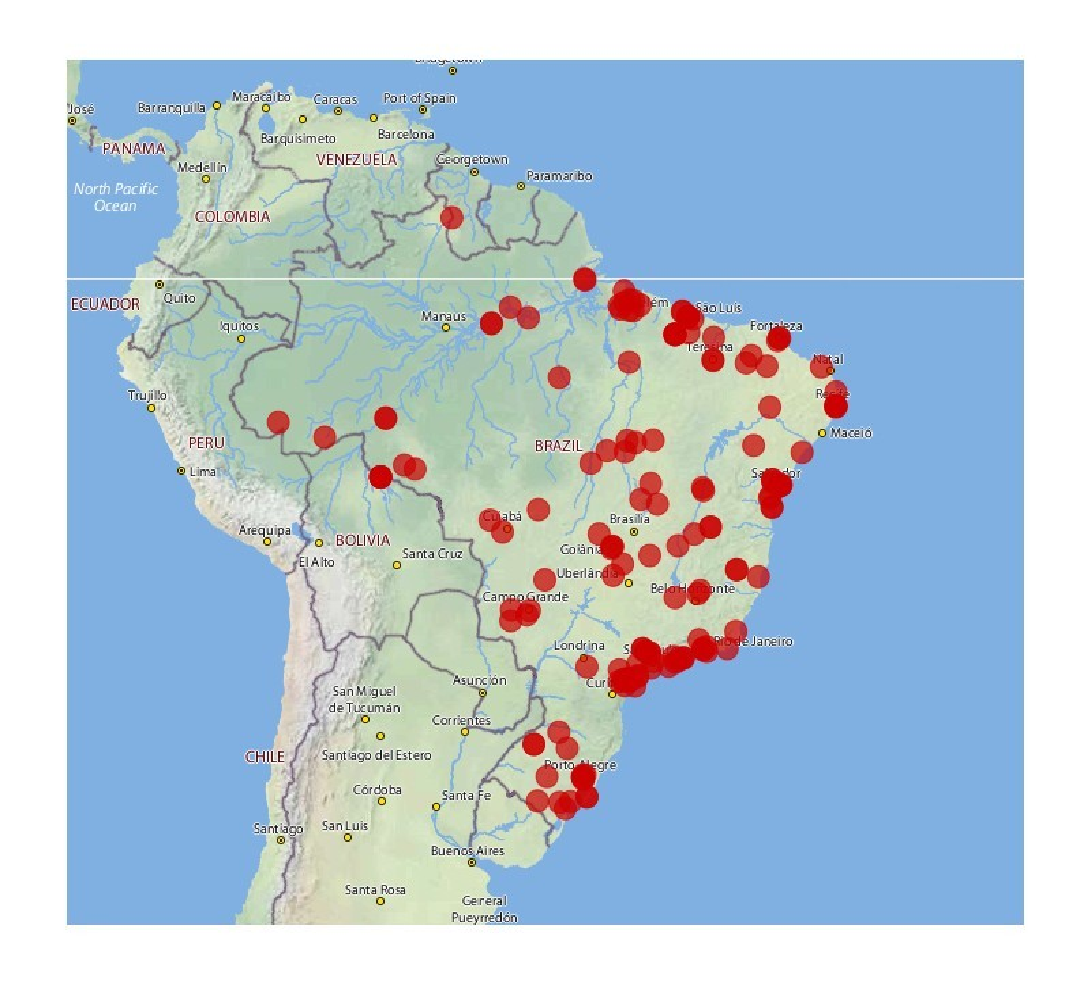
\includegraphics[width=\textwidth]{./Figure/MappaRedeMocambos.pdf}
  \rule{35em}{0.5pt}
  \caption[Mappa delle comunità della Rete Mocambos, tratto da
  \url{http://mapa.mocambos.net}]{Mappa delle comunità della Rete
    Mocambos, tratto da \url{http://mapa.mocambos.net}}
  \label{fig:MappaRedeMocambos}
\end{figure}

Il GESAC garantisce connettività satellitare a tutte le comunità, con
una banda limitata dovuta al tipo di tecnologia, non facilmente
sostituibile nel breve e medio termine. Tramite il programma
Telecentros.BR sono in corso di installazione dei \emph{telecentros},
sale attrezzate con computer ad accesso pubblico, e saranno erogate
borse per tutor locali, per la gestione degli spazi. Proprio in un
contesto così specifico nasce la necessità di adattare la tecnologia
alle esigenze locali, anche per le limitazioni tecniche imposte. La
scarsità di banda spinge a riconsiderare la rete non solo come il
mezzo di connessione verso i grandi \emph{data center}. La rete può, e
in questo caso deve, essere strutturata nel territorio con logiche di
sviluppo e gestione localmente determinate dalla comunità. In questo
senso è indispensabile la formazione e l'accesso alle tecnologie. La
\emph{Casa de Cultura Tainã}, nucleo fondatore della RM, è tra le
prime realtà popolari che hanno percepito la necessità del Software
Libero, come espressione della libertà di poter creare i propri
strumenti tecnologici digitali. L'esclusione digitale non riguarda
solo l'accesso al mondo digitale ma l'impossibilità di contribuire
alla sua creazione e crescita.

% \begin{figure}[htbp]
%   \centering
%   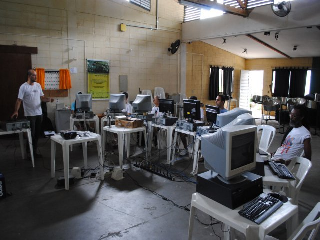
\includegraphics[width=\textwidth]{./Figure/taina_oficina.pdf}
%   \rule{35em}{0.5pt}
%   \caption[Laboratorio di grafica 3D con Blender alla \emph{Casa de
%     Cultura Tainã}]{Laboratorio di grafica 3D con Blender alla
%     \emph{Casa de Cultura Tainã}}
%   \label{fig:oficinaBlender}
% \end{figure}

\begin{figure}[htbp]
  \centering
  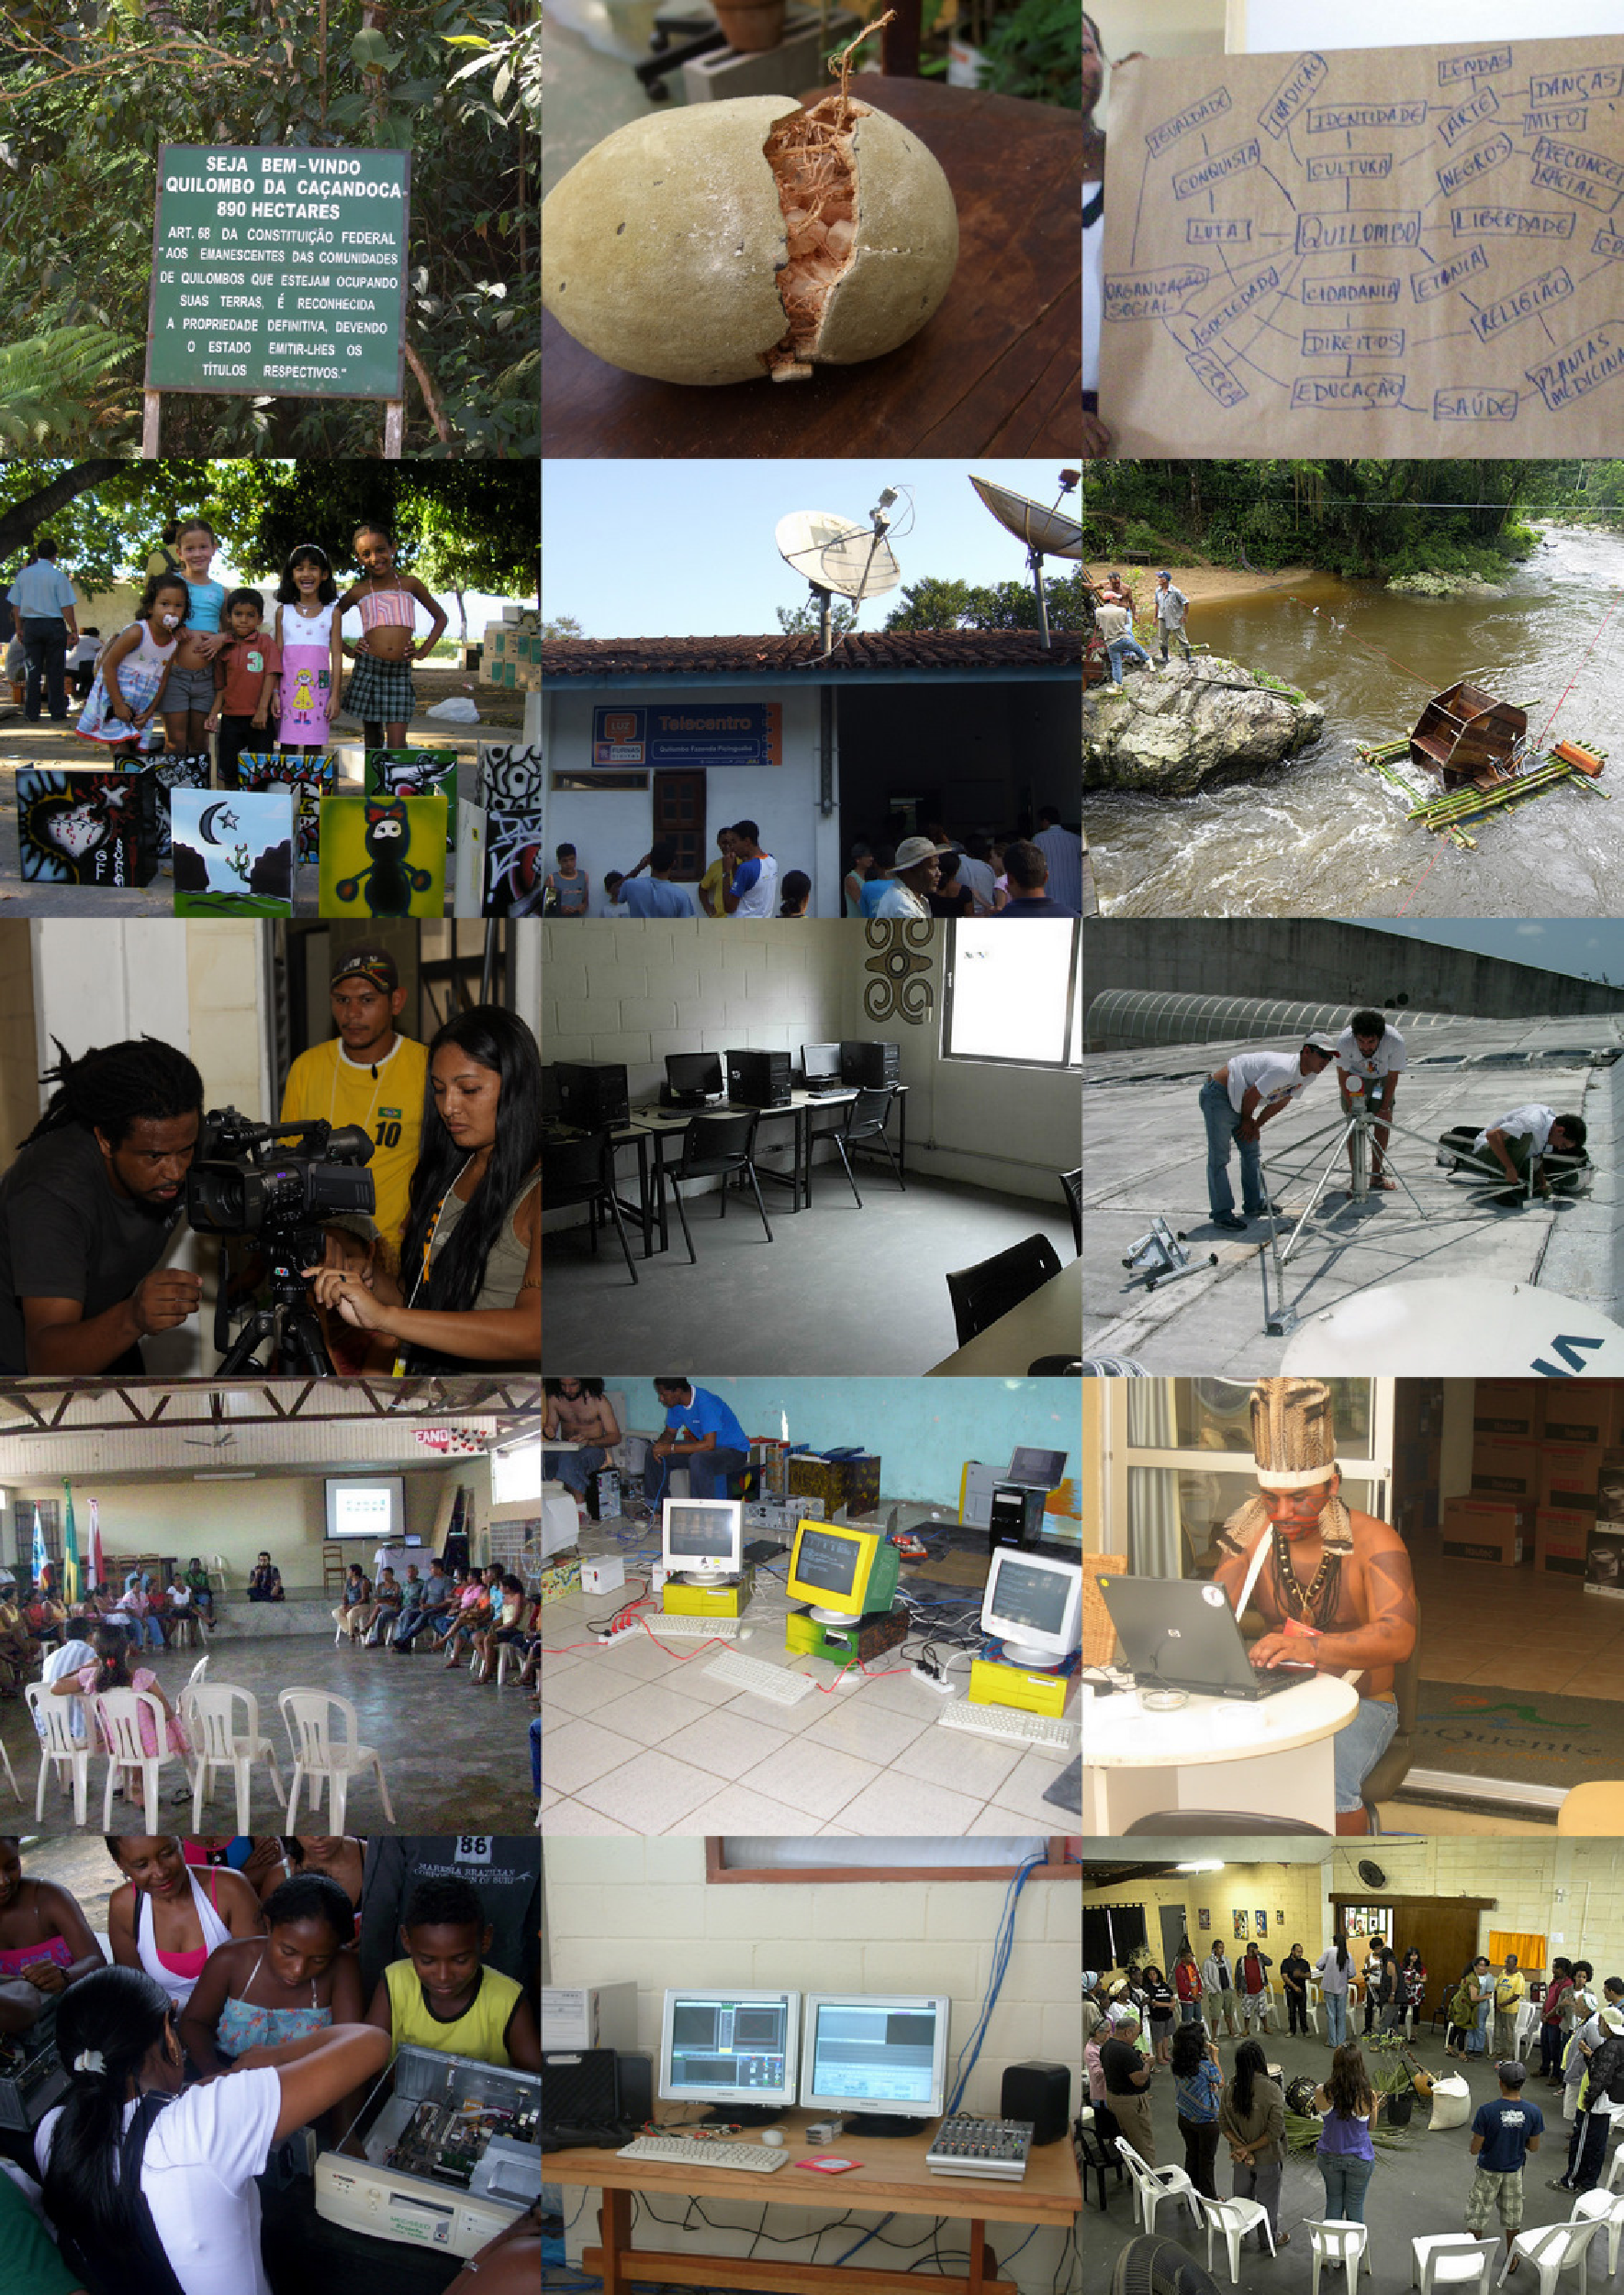
\includegraphics[width=\textwidth]{./Figure/FotoTesi.pdf}
  \rule{35em}{0.5pt}
  \caption[Composizione di foto della Rete Mocambos]{Composizione di
    foto della Rete Mocambos}
  \label{fig:FotoRM}
\end{figure}

Per la RM è importante, sotto molti aspetti, poter costruire e gestire
i mezzi di comunicazione e adattarli al loro contesto. In Brasile,
sono molte le comunità indigene, quilombola e
``tradizionali''\footnote{Per comunità tradizionali si intende
  comunità con culture e società proprie, per lo più di origine
  afro-indigena, situate spesso in ambito rurale e fortemente legate
  alla natura. La costituzione brasiliana sancisce il diritto alla
  terra per le comunità indigene e quilombola, e lo stato deve
  tutelare e garantire la diversità culturale.} che conoscono bene le
potenzialità delle tecnologie digitali e stanno, via via, cominciando
a dominarle. Ciò non sarebbe stato possibile senza l'esistenza e
l'ampia disponibilità di Software Libero. Tecnologie digitali sotto
forma di prodotti commerciali sarebbero un ennesimo passo verso la
dipendenza economica e culturale. Questa consapevolezza è alla base di
scelte ben ponderate. Ricordo che, qualche anno fa, a Brasilia,
durante una riunione del programma del governo federale \emph{Luz para
  Todos}, programma per fornire elettricità anche alla popolazione in
zone rurali e amene, un \emph{cacique}\footnote{ \emph{Cacique} è un
  termine con cui si definiscono i capi di alcune comunità indigene in
  America latina. } fece presente, che pur volendo l'energia
elettrica, questa dovesse essere limitata solo agli spazi comunitari e
non alle case. Non è difficile intuire il perché di tale
condizione. Oltre agli aspetti culturali, avere un contatore e una
bolletta per ogni casa significherebbe introdurre costi in denaro, che
non sono compatibili con la loro economia.

% \section{DA RIVEDERE}
% Una rete federata deve essere gestita. Servono risorse e conoscenze
% locali. Questo comporta un investimento strategico che riguarda
% aspetti ecomomici, ma sopratutto umani. E' necessaria una formazione
% continua e personale preparato per la gestione. Il mercato ha escluso
% questo modello anche per i suoi costi. Gli attori principali della
% new-economy globale sono riusciti a rendere questo passaggio quasi
% naturale, offrendo sistemi altamente funzionali e a condizioni
% particolarmente appetibili. Inanzitutto i servizi sono gratuiti e
% questo è la base per renderne l'uso in massa possibile. Da un punto di
% vista tecnico-informatico, la diffusione di servizi internet modello
% ToS vincenti, ha provocato una migrazione in massa delle maestrie del
% settore, sopratutto le nuove generazioni, verso lo sviluppo basato su
% API et similia.

% Passando dai protocolli di comunicazione standard alle API/ToS, dalla
% gestione della rete all'accesso al cloud, si p le conoscenze e
% sopratutto la ricerca

% (RITORNARE A DIRE PERCHE LE RETI FEDERATE SONO INTERESSANTI. SERVE UNA
% SCELTA POLITICA PER RIPRENDERE IL POSSESSO DELLA RETE COME SPAZIO
% TECNOLOGICO NON SOLO COME CONNESSIONE A POCHI CLOUD E DATACENTER)
% . Inoltre la programmazione di rete via API ha reso gli orizzonti in
% buona parte predeterminati dalle imprese madri del servizio.

% I nuovi mezzi di comunicazione offrono evidenti vantaggi, a cui non
% possiamo più rinunciare, tanto da spingere le Nazioni Unite a
% riconoscere l'accesso a internet come un diritto fondamentale \ref{}.

% Consideriamo in particolare una rete di servizi federati tra molte
% reti locali (attualmente circa 200 per la Rede Mocambos). La
% restrizione, oltre a essere dettata da un vincolo reale (la Rede
% Mocambos è basata su connessioni satellitari), può rappresentare un
% punto di partenza per ampliare la ricerca verso reti locali
% intelligenti e più sostenibili. Anche la diffusione di reti mesh ha
% risvegliato l'interesse per le reti di servizi federati su risorse
% decentralizzate e gestite localmente.


\section{Tecnologie}
Prima di addentrarci nei requisiti specifici, e nelle scelte adottate,
può essere utile una breve rassegna degli strumenti tecnologici in
varia misura utilizzati per strutturare il prototipo per la Rete
Mocambos di rete federata eventualmente connessa, in particolare per i
suoi servizi di base, quali identificazione, autenticazione e
messaggistica.

\subsection{LDAP}
Lightweight Directory Access Protocol (LDAP) è un insieme di
protocolli aperti per accedere a informazioni conservate centralmente
attraverso una rete. LDAP organizza le informazioni attraverso una
gerarchia ad albero chiamata Directory Information Tree (DIT). LDAP è
un sistema client/server. Il server può usare una varietà di database
per conservare un DIT, normalmente ottimizzati per le operazioni di
lettura. Quando un'applicazione client si collega ad un server LDAP,
può sia interrogare la directory che cercare di modificarla. Nel caso
in cui si verifica una interrogazione, il server può rispondere in
modo locale, oppure può inoltrare la richiesta ad un server LDAP che
sia in possesso di una risposta. Se l'applicazione di un client stà
cercando di modificare le informazioni all'interno di una directory
LDAP, il server verifica se l'utente possiede il permesso di
effettuare il cambiamento, e successivamente aggiunge o aggiorna le
informazioni. LDAP supporta la delega di parte del DIT a server
specifici, la replica in sola lettura e la replica in
lettura/scrittura (multi-master).  LDAP è un protocollo solido, molto
diffuso e supportato, e da tempo è lo standard de facto per gestire
basi di dati di utenti. OpenLDAP è una implementazione aperta e libera
del protocollo LDAP, che include client, server e una serie di
strumenti per facilitarne l'amministrazione.

\subsection{XMPP}
Extensible Messaging and Presence Protocol (XMPP) è un insieme di
protocolli aperti per la messaggistica e la presenza in rete basato su
XML. XMPP è un sistema client/server. Le specifiche per la
comunicazione tra server fanno si che gli utenti di un server possono
interagire in modo trasparente con gli utenti di altri server
federati. La XMPP Standards Foundation (XSF), coordina lo sviluppo
delle estensioni dello standard tramite le XMPP Extension Protocols
(XEPs), che ad oggi sono ben 311. XMPP e le XEPs costituiscono una
ambiente flessibile e completo per lo sviluppo di servizi
federati. Questi protocolli sono gia utilizzabili grazie a moltissime
implementazioni di server, client e librerie libere. Anche la storia
di XMPP, un tempo noto come Jabber, è interessante. Jabber venne
infatti inizialmente sviluppato da Jeremie Miller nella sua fattoria
nell'Iowa. E' un esempio concreto di come la ricerca e lo sviluppo di
tecnologie della comunicazione, fuori da ambiti accademici e
imprenditoriali, oltre che possibile può essere rivoluzionaria. Oggi
infatti XMPP è la tecnologia più usata per la messaggistica anche dai
grandi attori della new economy.

Per le necessità specifiche di una rete è possibile quindi estendere e
personalizzare le funzionalità del proprio server XMPP e al tempo
stesso usufruire dei servizi base, messaggistica e presenza,
implementanti dai server già esistenti in rete.

\subsection{OpenID}
OpenID è un sistema di identificazione decentralizzato nel quale la
propria identità è un URL che può essere verificata da qualunque
server supporti il protocollo. E' un protocollo aperto e sono
disponibili varie implementazioni libere. Inoltre il protocollo è
stato adottato dai principali fornitori di servizi web. Con OpenID è
possibile usare la stessa identità su piu servizi ed è un ottima base
per un sistema Single Sign On (SSO). Il protocollo sfrutta HTTP e e
Cookies per mantenere una sessione attiva. Al primo tentantivo di
autenticazione presso un servizio compatibile con OpenID, si viene
reindirizzati verso il proprio provider OpenID per effetturare
l'accesso e confermare l'autorizzazione a procedere al servizio
iniziale. Per tutta la durata della sessione, è possibile accedere ai
servizi OpenID senza reinserire le credenziali.

\begin{figure}[htbp]
  \centering
  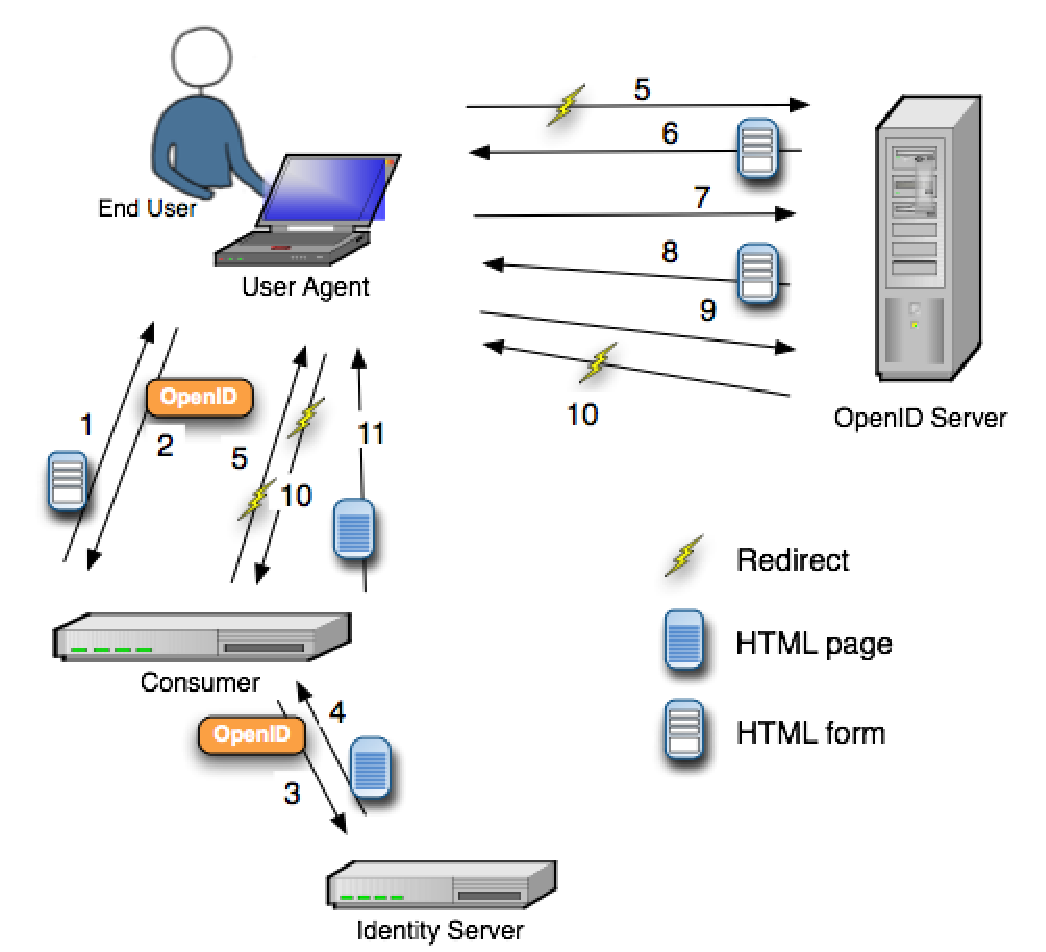
\includegraphics[width=0.6\textwidth]{./Figure/OpenID_Scenario.pdf}
  \rule{35em}{0.5pt}
  \caption[Diagramma di autenticazione di OpenID]{Diagramma di autenticazione di OpenID}
  \label{fig:OpenID}
\end{figure}



\subsection{OAuth}
OAuth è un protocollo aperto per l'autorizzazione di servizi tramite
API. Ad esempio, permette ad un utente di dare l'accesso alle sue
informazioni presenti su un sito detto service provider, ad un altro
sito, chiamato consumer, senza però condividere la sua identità. E' un
metodo per pubblicare e interagire con dati protetti. Esistono molti
altri protocolli e API simili come Google AuthSub, AOL OpenAuth, Yahoo
BBAuth, Upcoming API, Flickr API, Amazon Web Services e ognuno
fornisce dei metodi proprietari per lo scambio di credenziali e per
l'accesso tramite token. OAuth è una standardizzazione aperta delle
pratiche piu diffuse. Inoltre è stato pensato per il supporto a vari
tipi di applicazioni, non soltanto per i servizi web.


\subsection{Shibboleth}
Shibboleth è un architettura e un implementazione aperta per
l'autenticazione e autorizzazione di identità federate basata su
Security Assertion Markup Language (SAML). Le identità federate
permettono che le informazioni di un utente sotto un certo dominio
possano essere condividise con un altro dominio federato. Questo
permette il SSO attraverso piu domini senza lo scambio di nomi utente
e password. Gli IdP mantengono le informazioni sull'utente mentre i SP
fanno uso di queste informazioni per l'accesso sicuro ai contenuti.

\subsection{Kerberos}
Kerberos è un protocollo aperto per l'autenticazione forte in reti di
computer. E' un protocollo client/server e consente l'autenticazione
reciproca, ossia entrambi verificano le loro identità. Kerberos è
basato sul protocollo di Needham-Schroeder a chiavi simmetriche e
prevede un entità terza di fiducia chiamata Key Distribution Center
(KDC).

\subsection{Django}\label{Django}
Django è un framework, scritto in Python, per lo sviluppo rapido di
applicazioni web, anche conosciuto come ``\emph{The web framework for
  perfectionists with deadlines}''\footnote{``Il framework web per i
  perfezionisti con scadenze''.}, poichè è stato creato con l'obiettivo
di aderire il più possibile al principio DRY\footnote{``Don't Repeat
  Yourself (DRY, anche conosciuto come ``Single Point of Truth'') è un
  principio secondo il quale l'informazione non debba essere ripetuta
  e ridondante e non si debba esprimere lo stesso concetto più di una
  volta, specie se in forma diversa'', tratto da Wikipedia:
  \url{http://it.wikipedia.org/wiki/Don\%27t_Repeat_Yourself}.}, e
quindi fornisce tutti gli strumenti per scrivere codice pulito in modo
pragmatico ed efficace.

Le caratteristiche di Django sono le seguenti:
\begin{itemize}
\item Django è un framework \emph{Model, View, Template}, (MVT),
  corrispondente al diffuso pattern \emph{Model, View, Controller},
  (MVC). Il \emph{Template} di Django corrisponde alla \emph{view} in
  un qualunque framework MVC, mentre la \emph{View} corrisponde al
  \emph{controller} (anche se le funzionalità del \emph{controller},
  nel caso di Django, non sono limitate alla componente \emph{View}).
\item Django consente di modellare i dati direttamente in python e l'
  \emph{Object Relational Mapper}, (ORM), si occupa di trasformarli in
  codice SQL. Allo stesso modo non serve scrivere query direttamente
  in SQL; basta usare l'ORM per avere i risultati direttamente
  restituiti come oggetti python. L'ORM di Django supporta PostgreSQL,
  MySQL, sqlite, Microsoft SQL Server ed Oracle.
\item Django possiede una libreria per i \emph{forms} davvero potente ed
  espressiva, che consente di realizzare logiche complesse in poche
  righe di codice, lasciando il massimo controllo allo sviluppatore su
  ogni aspetto.
\item Django è un framework ``\emph{batteries included}'', ovvero
  contiene al suo interno alcune applicazioni, dette \emph{apps}, per
  le funzionalità più comuni che dimezzano il tempo di sviluppo, ad
  esempio un sistema di autenticazione, una interfaccia
  amministrativa, un framework per generare le \emph{sitemaps XML} e
  molto altro. Inoltre la \emph{community} è piuttosto attiva ed
  esistono molte \emph{apps} da adattare e riutilizzare.
\item Django è tra i migliori framework per quanto riguarda la
  documentazione ufficiale. Oltre ad alcuni tutorial, utili per
  impararne le basi, quasi ogni aspetto del framework è documentato in
  modo eccellente.
\end{itemize}

\subsection{Git}\label{sec:GIT}
Git è un sistema multi-piattaforma per il controllo delle versioni
distribuito, progettato per essere rapido e usabile anche in grandi
progetti.

Le caratteristiche principali includono:
\begin{itemize}
\item è totalmente distribuito e ogni clone di un
  \emph{repository} contiene l'intero storico delle versioni su cui
  possono essere effettuate operazioni indipendentemente da
  connessioni di rete o da server centrali. Le modifiche possono
  essere copiate da una clone all'altro e vengono mantenute su
  \emph{branch} diversi, facilitando le operazioni di \emph{merge}. I
  \emph{repository} sono facilmente accessibili tramite l'efficiente
  protocollo di Git che, oltre a supportare l'HTTP, può funzionare in
  combinazione con SSH, per avere connessioni sicure e un sistema di
  autenticazione solido e diffuso.
\item supporta il \emph{branching}, ramificazione, e il
  \emph{merging}, fusione, in modo rapido e conveniente, includendo
  una serie di strumenti per visualizzare e navigare lo storico non
  lineare delle versioni.
\item è molto veloce e scala bene quando si lavora con progetti
  molto grandi e con molte modifiche, grazie ad un efficiente sistema
  di pacchettizzazione e memorizzazione dello storico (è considerato
  il più efficiente tra i sistemi attualmente disponibili).
\item assegna un nome di versione, per ogni \emph{commit},
  che è funzione dell'intero storico, per cui una volta pubblicata una
  versione, non è possibile alterare le vecchie senza essere
  notati. Inoltre le versioni possono essere etichettate e firmate
  digitalmente tramite GPG.
\end{itemize}

Git è un sistema completo che, in buon stile Unix, è organizzato in
programmi e comandi indipendenti, pensati per essere facilmente
usabili, sia automaticamente tramite \emph{scripting} sia in modo
interattivo dall'utente finale. Git è, quindi, una base solida per lo
sviluppo di applicazioni orientate alla sincronizzazione, alla
portabilità, e alla gestione autonoma e decentrata.

 % Reti Federate  

\clearpage  % To start a new page

%% ----------------------------------------------------------------
% The "Funny Quote Page"
\pagestyle{empty}  % No headers or footers for the following pages

\null\vfill
% Now comes the "Funny Quote", written in italics
\textit{``A força da rede está nos nós''}

\begin{flushright}
TC
\end{flushright}

\vfill\vfill\vfill\vfill\vfill\vfill\null
\clearpage  % Funny Quote page ended, start a new page
%% ----------------------------------------------------------------

\pagestyle{fancy}  % Finally, use the "fancy" page style to implement
                   % the FancyHdr headers

% Capitolo 1

\chapter{Introduzione}
\label{Capitolo1}
\lhead{Capitolo 1. \emph{Introduzione}}

Questo lavoro parte da un esperienza diretta che ha avuto i natali nel
2004 a Firenze per poi svilupparsi e continuare in Brasile dal 2005 ad
oggi. Nel maggio del 2004, con il Collettivo di Informatica "Ada
Byron"\footnote{Il Collettivo di Informatica "Ada Byron", è un gruppo
  di studenti del Corso di Laurea in Informatica dell’Università degli
  Studi di Firenze. Il sito internet del collettivo è
  \url{http://informada.wordpress.com}.}, organizzammo una serie di
incontri e conferenze sul tema della libertà della conoscenza
applicata a vari ambiti. Parteciparono a "Modelli Liberi"\footnote{Un
  articolo sull'evento è disponibile su
  \url{http://www.apogeonline.com/webzine/2004/04/16/01/200404160103}.},
cosi si chiamarono gli incontri, relatori di rilievo internazionale,
quali Richard Stallman, Diego Saraiva, Juan Carlos Gentile e,
rappresentando il governo brasiliano, Sergio Amadeu e Elaine da
Silva. In seguito, nel 2005, mi trasferì a Brasilia dove iniziai a
lavorare al programma del governo federale brasiliano per
l'universalizzazione dell'accesso a internet, il GESAC (\emph{Governo
  Eletrônico Serviço de Atendimento ao Cidadão}). Il GESAC era, e
tuttora è, il più ambizioso progetto di lotta al \emph{digital divide}
dell'America Latina. Il programma prevedeva un numero iniziale di 3200
connessioni satellitari bidirezionali in tutto il territorio
nazionale, una piattaforma di servizi online e un equipe sul
territorio. Il Ministero delle Comunicazioni aveva affidato la
direzione del programma a Antonio Albuquerque, tra i fondatori del
Sindacato delle Telecomunicazioni brasiliano, che sostenne e diffuse
l'uso di Software Libero a tutti i livelli, sottolineandone
l'importanza strategica. Il nostro lavoro consisteva nella ricerca e
sperimentazione di soluzioni informatiche applicate ai più svariati
habitat e contesti sociali e culturali. Ci trovavamo continuamente a
contatto con realtà estremamente diverse. Il GESAC serve infatti
scuole, associazioni, caserme, comunità rurali, riserve indigene,
quilombo (Rif.), comunità di pescatori, ecc. Nella quasi totalità dei
casi erano persone alla prima esperienza informatica. L'approccio
scelto prediligeva il dialogo e il confronto aperto dove, ad esempio,
al posto di una lezione frontale, si ricorreva, ad esempio, ad una
\emph{roda de conversas}, tutti seduti in cerchio, pratica tra l'altro
molto popolare in Brasile. All'equipe del GESAC furono invitati a
lavorare persone con esperienza nell'ambito sociale, tra cui ad
esempio attivisti di Indymedia\footnote{``Indymedia e' un network di
  media gestiti collettivamente per una narrazione radicale, obiettiva
  e appassionata della verità. Ci impegniamo con amore e ispirazione
  per tutte quelle persone che lavorano per un mondo migliore, a
  dispetto delle distorsioni dei media che con riluttanza si impegnano
  a raccontare gli sforzi dell'umanità libera.'', tratto da
  http://www.indymedia.org/it/static/about.shtml .} e
Intervozes\footnote{``Intervozes è un'organizzazione che lavora per
  rendere effettivo il diritto umano alla comunicazione in Brasile.
  Per Intervozes, il diritto alla comunicazione è indissociabile dal
  pieno esercizio di cittadinanza e democrazia. Una società può essere
  definita democratica solo quando le diverse voci, opinioni e culture
  che la compongono hanno spazio per manifestarsi.'', tradotto da
  http://www.intervozes.org.br/o-intervozes .}. Il dialogo aperto e
paritario, a partire dalle specificità del contesto, apriva nuovi
spazi e punti di vista per la rivoluzione digitale, rimettendo al
centro della discussione il fine oltre che il mezzo. Non solo non
portavamo soluzioni preconfezionate, ma spesso gli strumenti e le
pratiche dovevano essere ridiscusse e possibilmente adattate a nuove
necessità.

\section{Neutralità tecnologica}
Questa tesi ricerca una soluzione tecnologica per facilitare la
comunicazione tra comunità quilombola. Queste comunità
afro-discendenti condividono tra loro molti aspetti sociali,
culturali, storici e geografici che le differenziano dalle realtà per
la quale, e dalla quale, sono sviluppati normalmente i mezzi di
comunicazione digitale. La neutralità del mezzo viene troppo spesso
data per scontata e risulta difficile percepire quanto questo in
realtà influisca e condizioni le nostre azioni e i nostri
obiettivi. Siamo portati a pensare al mezzo come neutrale, ma se
prendiamo ad esempio i principali e più diffusi mezzi di
comunicazione, le lingue, possiamo intuire come queste non siano
interscambiabili essendo l'espressione delle culture e delle società
che le usano e le vivono. Nell'era digitale è importante considerare
il peso e l'influenza dei nuovi linguaggi e mezzi di comunicazione.

\section{Internet, autonomia e libertà tecnologica}
Negli ultimi anni la diffusione della banda larga, ma sopratutto
strategie come quella adottata da Google, hanno trasformato il
concetto stesso di internet che da rete globale di reti eterogenee,
diventa principalmente una rete per la globalizzazione di servizi
fortemente centralizzati e uniformati. Fino a pochi anni fa era
normale per un'organizzazione provvedere alla gestione, mantenimento e
a volte allo sviluppo di servizi oltre che della infrastruttura
tecnologica per i propri utenti, a partire dalle basi di dati fino ai
servizi per la messaggistica. In questi contesti sono nati e si sono
sviluppate buona parte delle tecnologie di comunicazione oggi
disponibili ma che vengono in parte accantonate per scelte sopratutto
di mercato. Internet è nata dal confronto aperto tra i responsabili di
diverse reti, uniti dalla volontà di connettere le loro differenti
realtà. La nascita di nuovi servizi, per queste reti eterogenee, era
basata sulla discussione e il confronto. Il primo uso documentato del
termine "internet", seguendo questa pratica, fa la sua comparsa
proprio in un RFC \citep{RFC675}. I Request for comments (RFC), sono
dei documenti, normalmente scritti in un linguaggio semplice e
informale, mirati alla diffusione e discussione di nuove tecnologie
nell'ambiente delle telecomunicazioni. Sono anche la principale base
per la definizione di standard e protocolli. Attualmente è il canale
ufficiale di pubblicazione del \emph{The Internet Engineering Task
  Force (IETF)}, del \emph{The Internet Architecture Board (IAB)}, tra
le altre, e, in generale, della comunità mondiale dei ricercatori del
campo delle reti di comunicazione. Internet quindi, nata dalla pratica
della discussione, del confronto, della ``richiesta di commenti'', sta
ultimamente vivendo l'era dei \emph{Terms of Service (ToS)}. Ai
protocolli standard si sostituiscono API (Rif.) proprietarie e
suscettibili di alterazioni continue e unilaterali. Un impresa offre
servizi tramite API, decidendo i termini con cui gli utenti, o altre
imprese, possono accedere e utilizzare questi servizi.

In sostanza un tempo lo sviluppo seguiva un modello \emph{bottom up}, per
cui le maestranze informatiche sviluppavano sistemi ad hoc per le
esigenze locali, per poi in seguito aprire una discussione in rete,
con i loro corrispettivi, per definire dei protocolli standard e
mettere in comunicazione il tutto.

Oggi si passa ad un modello di sviluppo \emph{top down} per cui nuovi
servizi vengono lanciati basandosi su indagini di mercato e test su
campioni di utenti. Poche imprese fanno da padrone nel tracciare lo
sviluppo della rete che assume orizzonti sempre più determinati dal
mercato. Inoltre il mercato di riferimento, e il campione scelto, sono
per lo più legati al contesto economico, sociale e culturale
nordamericano e europeo. Pur essendo un analisi di interesse
filosofico/antropologico diventa territorio di frontiera con
l'informatica studiare la cultura digitale e gli effetti che le
tecnologie digitali possono avere sulle culture di paesi e popoli
diversi. Una analisi strutturata e analitica ci è stata lasciata da
Vilém Flusser, recentemente riscoperto e considerato tra i primi
filosofi della comunicazione dei nostri tempi, di cui riporto alcuni
pensieri pubblicati nel libro ``Towards a Philosophy of Photography'':

\begin{verbatim}
``Both those taking snaps and documentary photographers, however, have
not understood 'information.' What they produce are camera memories,
not information, and the better they do it, the more they prove the
victory of the camera over the human being.''
\end{verbatim}

\begin{verbatim}
``Our thoughts, feelings, desires and actions are being
robotized; 'life' is coming to mean feeding apparatuses and being fed
by them. In short: Everything is becoming absurd. So where is there
room for human freedom?''
\end{verbatim}

Un approccio diametralmente opposto alla centralizzazione della rete
sono le tecnologie Peer To Peer (P2P). Il principio base del P2P
prevede una infrastruttura di comunicazione in cui i nodi comunicano
direttamente tra di loro senza nodi centrali preconfigurati. Esistono
anche protocolli P2P che prevedono dei super-nodi, che in parte
riprendono il modello client/server, normalmente usati per ottimizzare
le prestazioni e risolvere problemi di attraversamento di reti
mascherate. In generale i sistemi P2P sono auto-configuranti o
necessitano di una conoscenza minima dell'architettura della rete
sottostante, dato che si basano su protocolli per l'instradamento
automatico dei pacchetti. Queste tecnologie funzionano bene quando un
numero sufficiente di nodi è attivo e partecipa al funzionamento della
rete. Un esempio di protocollo P2P molto diffuso è bittorrent, con cui
è possibile trasferire dati ad alte velocità quando i contenuti
richiesti sono presenti su nodi con banda a disposizione.

Nonostante le tecnologie P2P siano un alternativa disponibile e già
implementata a vari livelli, presentano alcune caratteristiche per cui
non sono applicabili al contesto della Rete Mocambos (RM) (vedi
\ref{sec:ReteMocambos}). Le connessioni tra le comunità della RM sono
tutte via satellite, con banda molto limitata. Un protocollo P2P,
gravando sulla banda di molti nodi per operazioni operate da un
singolo nodo, penalizzerebbe proprio la risorsa più scarsa.

Le necessità di una rete come la Rete Mocambos sono di vario tipo e gestite da
entità differenti sebbene federate. Nel prossimo capitolo vedremo un
tipo di rete federata per la RM. 

 % Introdução 

%% Capitolo 3

\chapter{Un'architettura per la Rete Mocambos}
\label{Capitolo3}
\lhead{Capitolo 3. \emph{Un'architettura per la Rete Mocambos}}

\section{Specifica dei requisiti}
La Rete Mocambos attualmente è composta da piu di 200 comunità
localizzate in tutto il territorio nazionale brasiliano e alcune
comunità in Africa e in Europa. La connettività in Brasile è
satellitare, garantita dal programma GESAC che mette a disposizione di
ogni comunità un Very Small Aperture Terminal (VSAT) con banda di 512
kbit/s in download e 128 kbit/s in upload. La topologia della rete è a
stella per cui tutti i nodi comunicano tramite satellite concentrando
il traffico su un hub terrestre, dove la rete satellitare è
interconnessa a Internet. Ogni comunità ha a disposizione una sala con
10 computer ad accesso pubblico, installati recentemente tramite il
Telecentros.BR\footnote{``Il programma nazionale di appoggio
  all'inclusione digitale nelle comunità, Telecentros.BR, è un'azione
  del Governo Federale di appoggio per la creazione di nuovi spazi
  pubblici e comunitari di inclusione digitale e per il potenziamento
  degli spazi già in funzione su tutto il territorio. Vengono messe a
  disposizione le apparecchiature informatiche e il mobiliario
  necessario al funzionamento dei \textit{telecentros}, servizi di
  connessione a internet tramite banda larga oltre a formazione e
  borse per l'appoggio economico per tutor che lavorano come agenti di
  inclusione digitale. Questi tutor borsisti partecipano ad un corso
  di formazione e lavorano, nei telecentros, per le comunità.'',
  tradotto da \url{http://www.inclusaodigital.gov.br/telecentros}.},
altro programma federale brasiliano. La popolazione di ogni comunità
varia dalle centinaia alle migliaia di persone. La maggior parte delle
comunità si trova in area rurale, spesso di difficile accesso e priva
di altri mezzi di comunicazione. A parte gli spazi comunitari,
normalmente concentrati in una zona centrale, la popolazione è divisa
in piccoli nuclei familiari sparsi sul territorio e a volte molto
distanti tra di loro.

Vediamo alcuni requisiti essenziali per questa architettura di rete
federata.

\subsection{Identità di rete}
Gli utenti delle comunità devono avere associate delle identità
digitali con cui accedere e utilizzare i servizi esistenti. Oltre ad
accedere localmente, è importante avere accesso ad alcuni servizi
anche al di fuori della propria comunità. Ad esempio, nel caso una
persona si trovi in città, deve poter accedere, attraverso internet,
ai servizi base, quale l'email, o ai portali e servizi web della
RM. È necessaria quindi un identità digitale di rete univoca.

\subsection{Autenticazione decentrata}
\label{sec:AutDec}
Un requisito essenziale per ogni comunità è l'autonomia in assenza di
collegamento ad internet, e la presenza quindi di un sistema locale di
autenticazione e autorizzazione. Oltre a garantire la continuità del
servizio (in relazione a problemi di connessione satellitare), è un
requisito importante per un buon disimpegno di tutti i servizi
autenticati.

\subsection{Sincronizzazione}
Lo scambio di informazioni tra le comunità è l'obbiettivo primario per
la RM. È quindi necessario un meccanismo per la sincronizzazione
selettiva dei contenuti di interesse generale. Inoltre, per
ottimizzare l'uso della banda, le operazioni di sincronizzazione dei
dati devono incidere il meno possibile sull'uso quotidiano di internet,
programmando queste operazioni per la notte o comunque quando la
connessione satellitare non è utilizzata. Il sistema deve prevedere
anche la possibilità di sincronizzare i dati da e verso periferiche di
archiviazione di massa.

\subsection{Riproducibilità}
Ogni comunità provvede autonomamente alla gestione della propria infrastruttura
tecnologica e le soluzioni adottate devono quindi essere facilmente
implementabili e adattabili localmente. Gli strumenti devono quindi essere
soluzioni stabili e possibilmente di uso comune, anche al fine di
reperire piu facilmente assistenza in loco. 

\subsection{Manutenzione}
La manutenzione del sistema deve prevedere sia interventi a distanza
sia locali. Il sistema deve essere basato su tecnologie standard e
aperte per garantire l'accesso ai dati anche in caso di problemi.

\subsection{Sviluppo}
Ogni comunità ha caratteristiche e necessità proprie che portano alla
richiesta di servizi differenziati. L'architettura generale della RM
deve essere una base stabile su cui poter sviluppare servizi senza
vincoli troppo stringenti. Le tecnologie e i linguaggi adottati devono
facilitare l'interazione, la formazione e il riuso delle conoscenze. 

\section{Strumenti e pratiche per lo sviluppo}
Data la natura della RM, e in particolare la necessita di autonomia
tecnologica, la formazione è fondamentale per cui è importante l'uso
di strumenti che facilitino la documentazione e lo sviluppo
collettivo. La RM utilizza già da anni un wiki\footnote{``Una Wiki è
  una pagina (o comunque una collezione di documenti ipertestuali) che
  viene aggiornata dai suoi utilizzatori e i cui contenuti sono
  sviluppati in collaborazione da tutti coloro che vi hanno
  accesso. La modifica dei contenuti è aperta, nel senso che il testo
  può essere modificato da tutti gli utenti (a volte soltanto se
  registrati, altre volte anche anonimi) contribuendo non solo per
  aggiunte come accade solitamente nei forum, ma anche cambiando e
  cancellando ciò che hanno scritto gli autori precedenti.  Ogni
  modifica è registrata in una cronologia che permette in caso di
  necessità di riportare il testo alla versione precedente; lo scopo è
  quello di condividere, scambiare, immagazzinare e ottimizzare la
  conoscenza in modo collaborativo. Il termine wiki indica anche il
  software collaborativo utilizzato per creare il sito web e il
  server.'', tratto da \url{http://it.wikipedia.org/wiki/Wiki}.},
disponibile all'indirizzo \url{http://wiki.mocambos.net}, dove è
disponibile, in lingua portoghese, una parte della documentazione sul
codice sviluppato per questo lavoro. Per il versionamento del codice
del lavoro svolto si è scelto di usare il sistema decentrato GIT (vedi
\ref{sec:GIT}) e la piattaforma
GITHUB\footnote{\href{http://github.com}{GITHUB} è una rete sociale
  basata sul sistema GIT \ref{sec:GIT}.}. Il codice del prototipo è
disponibile all'indirizzo \url{https://github.com/RedeMocambos}

\subsection{Sistema operativo}
La scelta di un sistema operativo comune facilita la documentazione,
l'automazione e l'assistenza a distanza. Molte comunità utilizzano già
distribuzioni GNU\\Linux basate su Debian\footnote{``Il Progetto
  Debian è una associazione di persone che ha come scopo comune la
  creazione di un sistema operativo libero. Il sistema operativo che
  abbiamo creato si chiama Debian GNU/Linux, o semplicemente
  Debian.'', tratto da \url{http://www.debian.org/}}. Per il prototipo
sono state scelte l'ultima versione stabile, di Debian, la 6.0, e di
Ubuntu\footnote{``Ubuntu è un sistema operativo GNU\/Linux nato nel
  2004, basato su Debian, che si focalizza sull'utente e sulla
  facilità di utilizzo. Ubuntu è orientato all'utilizzo desktop e pone
  una grande attenzione al supporto hardware. È prevista una nuova
  versione ogni sei mesi.  Finanziato dalla società Canonical Ltd
  (registrata nell'Isola di Man), questo sistema è rilasciato come
  software libero sotto licenza GNU GPL ed è gratuito e liberamente
  modificabile.'', tratto da
  \url{http://it.wikipedia.org/wiki/Ubuntu}.}, la 11.10.

\subsection{Linguaggi di programmazione}
Per il sistema sviluppato si è scelto l'uso del linguaggio di
programmazione Python, un linguaggio molto flessibile e probabilmente
il più versatile per connettere componenti eterogenee. Inoltre alcune
comunità già usano Software Liberi, quali
\emph{GIMP}\footnote{\emph{GNU Image Manipulation Program (GIMP)} è un
  programma per il fotoritocco, montaggio e creazione di
  immagini. Disponibile su \url{http://www.gimp.org/}.},
\emph{Blender}\footnote{\emph{Blender} è un programma per la creazione
  di grafica e ambienti tridimensionali. Disponibile su
  \url{http://www.blender.org/}.},
\emph{Inkscape}\footnote{\emph{Inkscape} è un programma di grafica
  vettoriale conforme allo standard SVG. Disponibile su
  \url{http://inkscape.org}.} che fanno ampio uso di \emph{scripting}
Python per la creazione di filtri e per altre funzionalità avanzate.

\subsection{Virtualizzazione}
Il prototipo è stato sviluppato e testato in un ambiente
virtualizzato, per garantire maggior controllo e verificare la
correttezza del procedimento in tutti i suoi passaggi. Gli
\emph{script} per automatizzare le installazioni, e le procedure passo
passo presenti nella documentazione, sono state eseguite a partire da
un sistema base. Sono state create delle macchine virtuali, con
l'aiuto del programma libero
\emph{VirtualBox}\footnote{\emph{VirtualBox} è un virtualizzatore
  completo per architettura x86 per l'uso in server, computer
  personali e sistemi \emph{embedded}. Dispobibile su
  \url{http://www.virtualbox.org/}.}, simulando dei server
comunitari/locali e il server centrale.


\section{Architettura di base}

\subsection{Gestione delle identità di rete}
Analizzando la specifica dei requisiti e alcune delle tecnologie
esistenti viste nel capitolo precedente, è stato scelto l'uso di LDAP
per gestire le credenziali degli utenti all'interno della RM. Il
prototipo proposto prevede un server centrale su connettività internet
garantita e server locali in replica. È possibile pensare una
configurazione in cui tutti i server della rete sono configurati in
modalità N-Way-Multimaster. Questa configurazione, se da un lato
consente l'aggiornamento in scrittura della base utenti su ognuno dei
server, può generare più facilmente situazioni di inconsistenza dei
dati e problemi di sincronizzazione tra i server LDAP. Per questo
motivo per il prototipo realizzato si è scelto di rilassare il
requisito \ref{sec:AutDec}, ipotizzando un singolo server master per
tutta la rete su cui effettuare le operazioni in scrittura (creazione,
eliminazione e aggiornamento di utenti) e server locali abilitati solo
ad operazioni in lettura. Ogni comunità quindi avrebbe a disposizione
un server LDAP in replica su cui basare le operazioni di
autenticazione e autorizzazione. In mancanza di connessione esterna i
servizi locali rimangono comunque attivi per le utenze attive fino
all'ultima sincronizzazione.


\subsection{Mocambos\_LDAP}
\framebox[\textwidth]{\footnotesize Il codice è disponibile su
\url{https://github.com/RedeMocambos/Mocambos_LDAP}}

Per facilitare l'implementazione dei server LDAP dagli amministratori
locali è stato sviluppato uno script di installazione, che può tornare
utile anche per un amministratore remoto.

Lo script \textit{bash} provvede ad installare i pacchetti necessari e
preparare il server LDAP \emph{slapd} in configurazione master o
replica. Inoltre crea un DIT preconfigurato per la RM con una semplice
struttura (vedi figura \ref{fig:DIT_ReteMocambos}).

\begin{figure}[htbp]
  \centering
  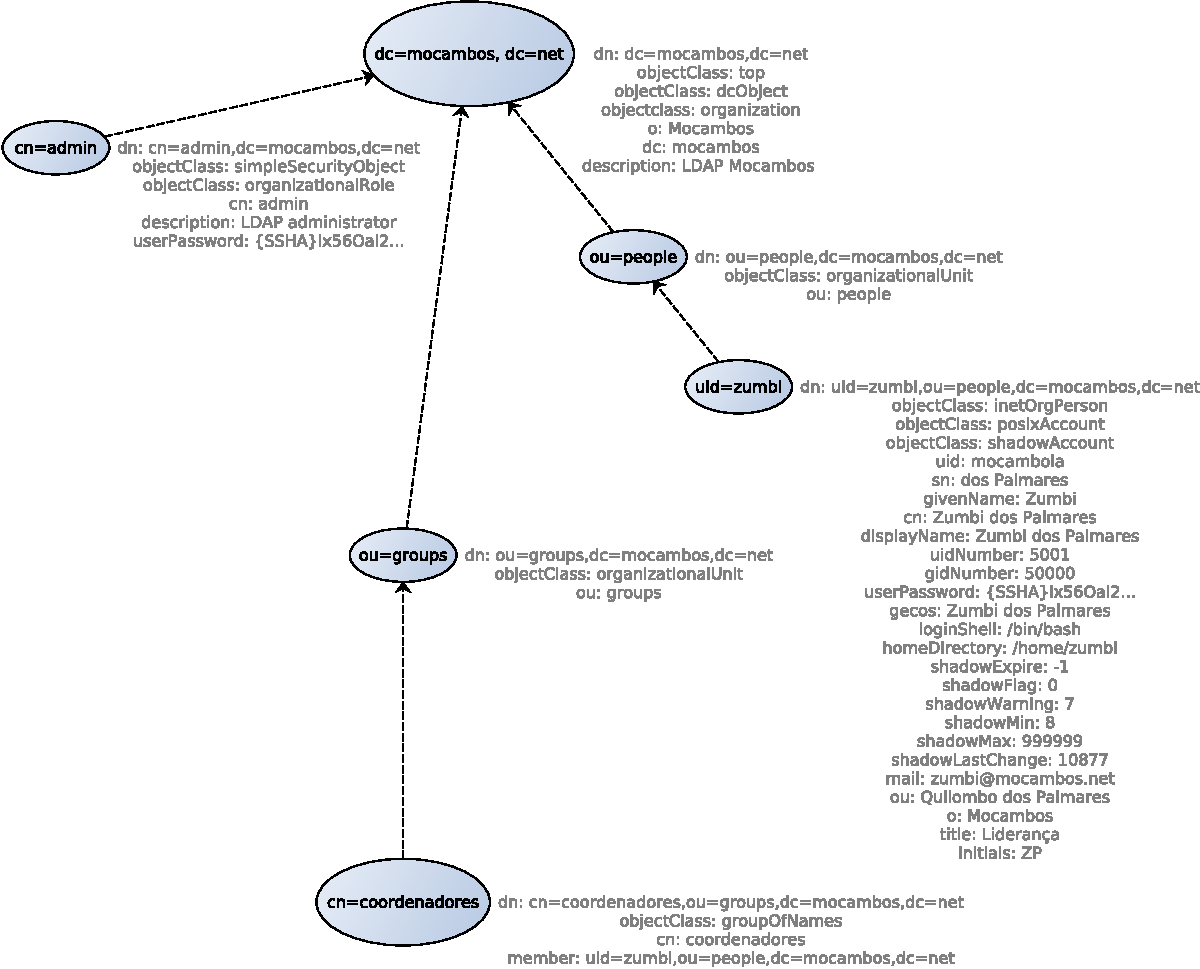
\includegraphics[width=\textwidth]{./Figure/DIT_ReteMocambos-crop.pdf}
  \rule{35em}{0.5pt}
  \caption[DIT di base del server LDAP della RM]{DIT di base del
    server LDAP della RM.}
  \label{fig:DIT_ReteMocambos}
\end{figure}




 % Architettura

%% Capitolo 4

\chapter{Un prototipo di servizio federato}
\label{Capitolo3}
\lhead{Capitolo 3. \emph{Un prototipo di servizio federato}}

\section{Sistema di pubblicazione e diffusione di contenuti
  multimediali}
L'uso delle tecnologie digitali offre nuove possibilità per
l'educazione. Molte comunità afferenti alla RM hanno iniziato la
produzione di materiale pedagogico audio-visuale che con l'aiuto della
rete potrebbe contribuire ad arricchire i programmi educativi pubblici
spesso carenti e poco integrati con la cultura quilombola. Da
tempo\footnote{Il progetto \emph{Tambor e Comunicação} é un tentativo
  di fortificare la rete di comunicazione digitale per le necessità
  delle comunità. Vedi
  \url{http://wiki.mocambos.net/wiki/Projeto_Tambor_e_Comunicacao}.},
quindi, il \emph{Núcleo de Pesquisa e Desenvolvimento Digital
  (NPDD)}\footnote{Il \emph{Núcleo de Pesquisa e Desenvolvimento
    Digital (NPDD)} della RM ricerca e sviluppa tecnologie digitali
  per la comunicazione, la produzione di energie rinnovabili e
  sostenibili, e il miglioramento delle condizioni di vita in simbiosi
  con l'ambiente. Maggiori informazioni su
  \url{http://wiki.mocambos.net/wiki/NPDD}.} nucleo di ricerca e
sviluppo digitale della RM cerca una soluzione per la pubblicazione e
diffusione in rete di immagini, audio e video di interesse comune e
spesso prodotti nelle stesse comunità. Il sistema prevede
l'installazione di un portale sul server locale delle comunità su cui
è possibile pubblicare contenuti multimediali sfruttando l'alta
velocità della rete locale. Il sistema si prende cura di diffondere i
contenuti, etichettati come di interesse comune, verso i server delle
altre comunità. Il prototipo sviluppato cerca di risolvere le
limitazioni di banda della rete rispettando la specifica di requisiti.

\section{Portale Comunitario}
Per lo sviluppo di un portale locale è stato scelto l'uso di Django.


 % Prototipo

%% Capitolo 4

\chapter{Conclusioni e sviluppi futuri}
\label{Capitolo5}
\lhead{Capitolo 5. \emph{Conclusioni e sviluppi futuri}}

L'architettura e il prototipo sviluppato saranno implementati su scala
ridotta a partire dalle comunità più strutturate e che fungono già da
poli regionali, chiamati \emph{Nucleos de Formação Continuada, (NFC)},
Nuclei di Formazione Continua, che sono attualmente dieci e
geograficamente ben distribuiti sul territorio nazionale brasiliano.

Il codice prodotto consente una prima implementazione per un progetto
pilota che coinvolga sviluppatori del NPDD e consenta la formazione di
tecnici locali nei NFC, oltre ad un feedback diretto di uso da parte
delle comunità. 

Attualmente il codice supporta:
\begin{itemize}
\item autenticazione LDAP (gestione basica dei gruppi)
\item creazione e upload di contenuti audio, video e immagini
\item distribuzione tramite git-annex
\item sincronizzazione degli oggetti sui portali django (ricreando gli
  oggetti distribuiti via git-annex)
\end{itemize}

% \begin{figure}[htbp]
%   \centering
%   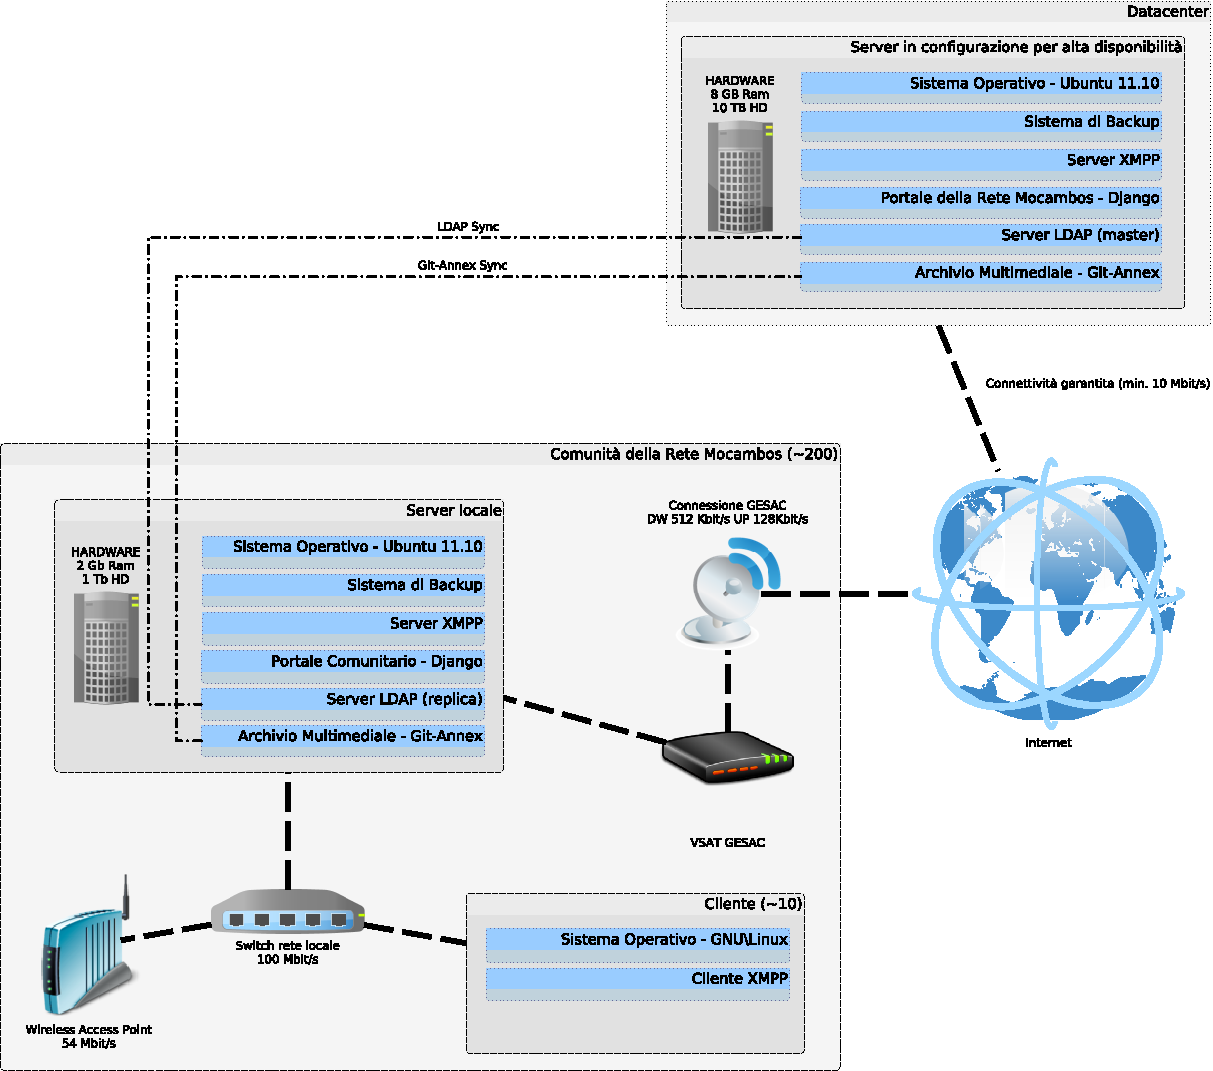
\includegraphics[width=\textwidth]{./Figure/SchemaServer_ReteMocambos-crop.pdf}
%   \rule{35em}{0.5pt}
%   \caption[Schema dell'infrastruttura della RM]{Schema dell'infrastruttura della RM.}
%   \label{fig:SchemaServer_ReteMocambos}
% \end{figure}
 % Conclusioni

%\input{./Chapters/Chapter6} % Results and Discussion

%\input{./Chapters/Chapter7} % Conclusion

%% ----------------------------------------------------------------
% Now begin the Appendices, including them as separate files

\addtocontents{toc}{\vspace{2em}} % Add a gap in the Contents, for aesthetics

\appendix % Cue to tell LaTeX that the following 'chapters' are Appendices

% Appendice A                                                                                                                                                                   
\chapter{Listato del codice}
\label{AppendiceA}
\lhead{Appendice A \emph{Listato del codice}}

% \lstset{frame=tb,
%   language=Python,
%   aboveskip=3mm,
%   belowskip=3mm,
%   showstringspaces=false,
%   columns=flexible,
%   numbers=none,
%   numberstyle=\tiny\color{gray},
%   keywordstyle=\color{blue},
%   commentstyle=\color{dkgreen},
%   stringstyle=\color{mauve},
%   breaklines=true,
%   breakatwhitespace=true
%   tabsize=2
%   basicstyle={\scriptsize\ttfamily},
%   morekeywords={models, lambda, forms, =}
%   multicols=2
% }

\section{gitannex}

\subsection{gitannex/admin.py}
\lstinputlisting[basicstyle={\scriptsize\ttfamily}]{src/gitannex/admin.py}

\subsection{gitannex/models.py}
\lstinputlisting[basicstyle={\scriptsize\ttfamily}]{src/gitannex/models.py}

\subsection{gitannex/signals.py}
\lstinputlisting[basicstyle={\scriptsize\ttfamily}]{src/gitannex/signals.py}

\subsection{gitannex/management/commands/run scheduled jobs.py}
\lstinputlisting[basicstyle={\scriptsize\ttfamily}]{src/gitannex/management/commands/run_scheduled_jobs.py}


\section{mmedia}

\subsection{mmedia/admin.py}
\lstinputlisting[basicstyle={\scriptsize\ttfamily}]{src/mmedia/admin.py}

\subsection{mmedia/models.py}
\lstinputlisting[basicstyle={\scriptsize\ttfamily}]{src/mmedia/models.py}

\subsection{mmedia/signals.py}
\lstinputlisting[basicstyle={\scriptsize\ttfamily}]{src/mmedia/signals.py}

\subsection{mmedia/forms.py}
\lstinputlisting[basicstyle={\scriptsize\ttfamily}]{src/mmedia/forms.py}

\subsection{mmedia/management/commands/create objects from files.py}
\lstinputlisting[basicstyle={\scriptsize\ttfamily}]{src/mmedia/management/commands/create_objects_from_files.py}
	% Appendice codice sorgente

%\input{./Appendices/AppendixB} % Appendix Title

%\input{./Appendices/AppendixC} % Appendix Title

\addtocontents{toc}{\vspace{2em}}  % Add a gap in the Contents, for aesthetics
\backmatter
\nocite{*}
%% ----------------------------------------------------------------
\label{Bibliography}
\lhead{\emph{Bibliography}}  % Change the left side page header to "Bibliography"
\bibliographystyle{unsrtnat}  % Use the "unsrtnat" BibTeX style for formatting the Bibliography
\bibliography{Bibliography}  % The references (bibliography) information are stored in the file named "Bibliography.bib"

\end{document}  % The End
%% ----------------------------------------------------------------
